\chapter{Nitrogen}
\label{chap:n2}
\section{Recent developments}
            Experimental second virial coefficients have often complemented \abinitio{} PESs for nitrogen that have resulted in rescaled or improved PESs. With the advent of computational techniques we expect that theory is soon to replace experiments as the source of high quality virial coefficients (see e.g. Shaul et al. \cite{Shaul2012SC} for the case of helium-4). Such highly accurate and precise second virial coefficient data will lead to better quality PESs, using which one can predict thermodynamic, transport, structural and other properties of nitrogen much more accurately. Berns and van der Avoird \cite{Berns1980} reported one of the first \abinitio{} PES (BvdA) for the Nitrogen (${\rm N_2 - N_2}$) dimer including first order exchange, short-range electrostatic contributions and long-range data of Mulder et al. \cite{Mulder1980}. They developed two analytic representations of their calculations: 1) A spherical harmonic expansion and 2) a two site point charge model with a shifted force center. Describing the region near the van der Waals minimum accurately, was one of the primary goals of their work. The BvdA potential was used to study crystal structure properties \cite{Luty1980} and transport properties \cite{Nyeland1984}. Whereas the long-range interaction calculations performed by Mulder et al. \cite{Mulder1980} were obtained using uncoupled HF method, Visser et al. \cite{Visser1983} performed time-dependent coupled HF method and consequently reported more accurate long-range interaction coefficients. Ad van der Avoird et al. \cite{vanDerAvoird1986} reported a new potential(AWJ) by including these improved long-range coefficients and more basis sets. However, it was observed that the van der Waal well prediction of the potential was too shallow. This resulted in large discrepancies between the calculated second virial coefficient values and the experimentally observed results. Neglect of intramolecular electron correlation leading to significant short-range exchange repulsion in the intermolecular potential was identified and later confirmed to be the possible cause for this discrepancy. Therefore, they introduced two scaling constants to change the size and slope of the short-range exchange repulsion term to obtain a rescaled potential that yielded second virial coefficients that were in much better agreement with experiments. Highly accurate experimental virial coefficient data sets were used to improve \abinitio{} PES obtained as a result of calculations performed at the CCSD(T) level with large basis sets by Stallcop et al. \cite{Stallcop1997}. A semi-empirical relation between the parameters of the repulsive potential and the accurate virial coefficient data sets was also reported. Cappelletti et al. \cite{Cappelletti1998} also reported a potential which was an improvement of the AWJ potential, by firstly computing \abinitio{} PES at the CCSD(T) level of theory and then using accurate data from scattering, virial coefficients and other property measurements to improve the PES quality. An extensive \abinitio{} study was conducted by Leonhard et al. \cite{Leonhard2002} to not only develop a improved 2-body potential but also to analyze two 3-body potentials for their capability to reproduce thermodynamic properties if both the 2-body as well as 3-body potentials were used. The 2-body \abinitio{} PES was rescaled to fit accurate second virial coefficient data. After comparison to experimental results, the 3-body potential due to Axilrod Teller (AT) \cite{Axilrod1943} performed better than the one due to Stogryn \cite{Stogryn1969}, when used in combination with the 2-body potential. Gomez et al. \cite{Gomez2007} reported an \abinitio{} PES that was calculated using SAPT. The accuracy of perturbative energies were compared against calculations at the CCSD(T) level of theory using large basis sets. They observed better agreement to experimental virial coefficients than previous unscaled PESs for the range of temperatures investigated. They attributed the consistently lower second virial coefficient predictions by using their PES, to possible overestimation of the van der Waal's well within their calculations. Str\k{a}k et al. \cite{Strak2007} also performed \abinitio{} calculations at the CCSD(T) level of theory that resulted in a potential that was used in combination with Molecular Dynamics (MD) simulations to obtain an equation of state for the dimer. The resulting predictions of physical properties based on this equation of state were found to be in excellent agreement with experiments for a wide range of temperatures (up to 2000K) and pressures (up to 30GPa). Hellmann \cite{Hellmann2013} recently performed \abinitio{} calculations at the CCSD(T) level of theory using basis sets up to aug-cc-pV5Z supplemented with bond functions. The resulting 2-body (scaled) and 3-body potential was used to compute second and third (including 3-body effects) virial coefficients that were most accurate with experiments than previously reported values.
\section{Computational details}
    \subsection{Second virial coefficients}
    \label{subsubsec:b2n2}
        The \abinitio{} potential (denoted as $U_2^H$) that we used was due to Hellmann \cite{Hellmann2013}. We have performed classical and semi-classical virial coefficient calculations, each using $10^9$ configuration samples and two types of MC trials 1) translation and 2) rotation of the dimer. Instead of using the semi-classical TI version of the Hellmann potential, we have used the semi-classical QFH version of the potential which is given as follows \cite{Feynman,Schenter2002}:
        \begin{equation}
        \label{eq:QFH}
            U_2^{\rm QFH} = U_2^H + \displaystyle\frac{\hbar^2 \beta}{24 m} \Big[ \pmb{\nabla}^2 U_2^H + \frac{2}{r} \pmb{\nabla} U_2^H \Big].
        \end{equation}

        This was done based on some preliminary calculations that we carried out where we failed to observe any significant improvement in the precision of the results while using the semi-classical TI version of $U_2^H$ (which was done by Hellmann). Therefore we expect significant differences while comparing our virial coefficient values for the semi-classical calculations against Hellmann's, especially at low temperatures. We have performed PIMC calculations using $P$ = 8, 16, 32 and 64 classical images for each of the temperatures reported by Hellmann and collected $10^8$ configuration samples each. Apart from the translation of the dimer, we also include MC trials to regrow the ring by translating the beads (see Sec. \ref{subsec:orMove}) and our recently developed orientation algorithm (cite:hydrogen) (explained in Sec. \ref{subsec:orMove}). We have performed PIMC calculations using semi-classical images and also the exact same conditions as PIMC with classical beads that are mentioned above. We note that for this calculation, we employed the TI propagator (Eq. \eqref{eq:TI}).

    \subsection{Third virial coefficients}
        We repeated all the calculations under the same conditions (except the semi-classical additive as well as non-additive calculations for which we used $10^8$ configuration samples as opposed to $10^9$ for the second virial coefficient case) that were explained in Sec. \ref{subsubsec:b2n2} for computing the additive as well as non-additive contributions to the third virial coefficients. It should be noted that we employed the non-additive 3-body potential that was also reported by Hellmann \cite{Hellmann2013} to compute the non-additive contributions. Also, we performed the semi-classical additive as well as non-additive simulations using the same QFH version of $U_2^H$ as in Eq. \eqref{eq:QFH}. We note that all the third virial coefficient simulations were performed at a set of 90 temperatures considered by Hellmann.
\section{Results and discussion}
    \subsection{Second virial coefficients}
        In order to reproduce the results of Hellmann and to ensure that our implementation of the \abinitio{} potential was correct, we performed classical virial coefficient calculations as a first step. In Fig. \ref{fig:B2CLN2} we show the difference, between our results and Hellmann's for the second virial coefficient as a function of temperature, in the main plot and show the actual values in the inset plot, also as a function of temperature.
        \begin{figure}[!htbp]
            \centering
            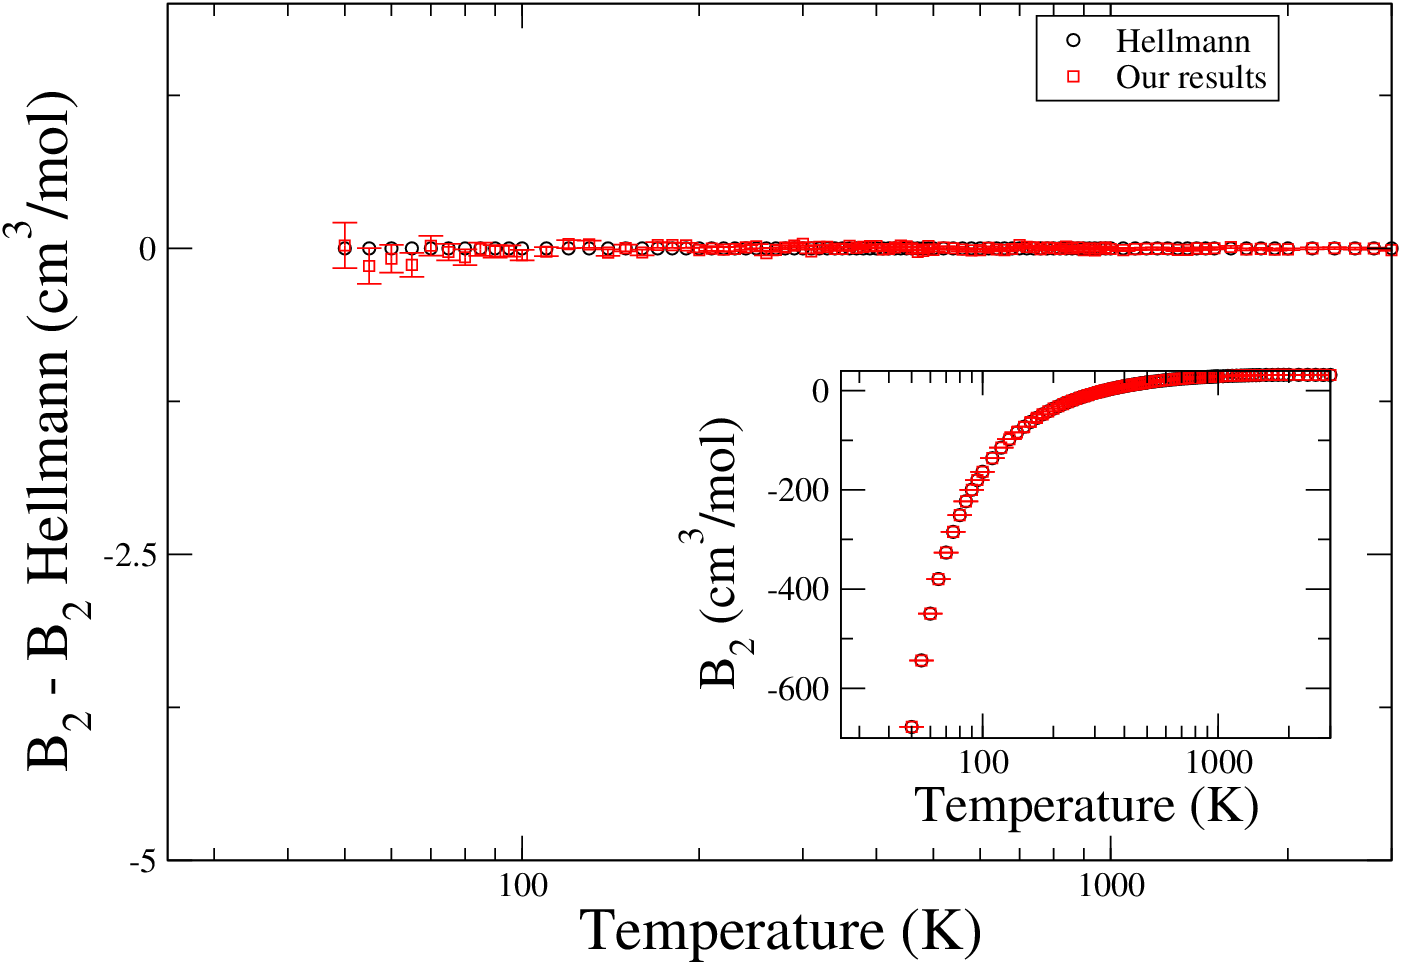
\includegraphics[scale=0.20,keepaspectratio]{Chapter-5/Figures/B2CL9sResultsAll.png}
            \caption{Classical second virial coefficient ($B_2$) values compared against Hellmann's values \cite{Hellmann2013}. Error bars are drawn at $\mu \pm \sigma$ where $\mu$ is the mean value and $\sigma$ is the standard error. It should be noted however, that the 95\% confidence interval is given by $\mu \pm 2\sigma$.}
            \label{fig:B2CLN2}
        \end{figure}
        It can be clearly seen from Fig. \ref{fig:B2CLN2} that our classical results are in excellent statistical agreement with Hellmann's for the entire range of temperatures, suggesting that our implementation of the \abinitio{} potential is correct.

        In Fig. \ref{fig:B2SCN2} we show the difference between, our semi-classical second virial coefficient results and Hellmann's as a function of temperature, in the main plot and show the actual values in the inset plot, also as a function of temperature.
        \begin{figure}[!htbp]
            \centering
            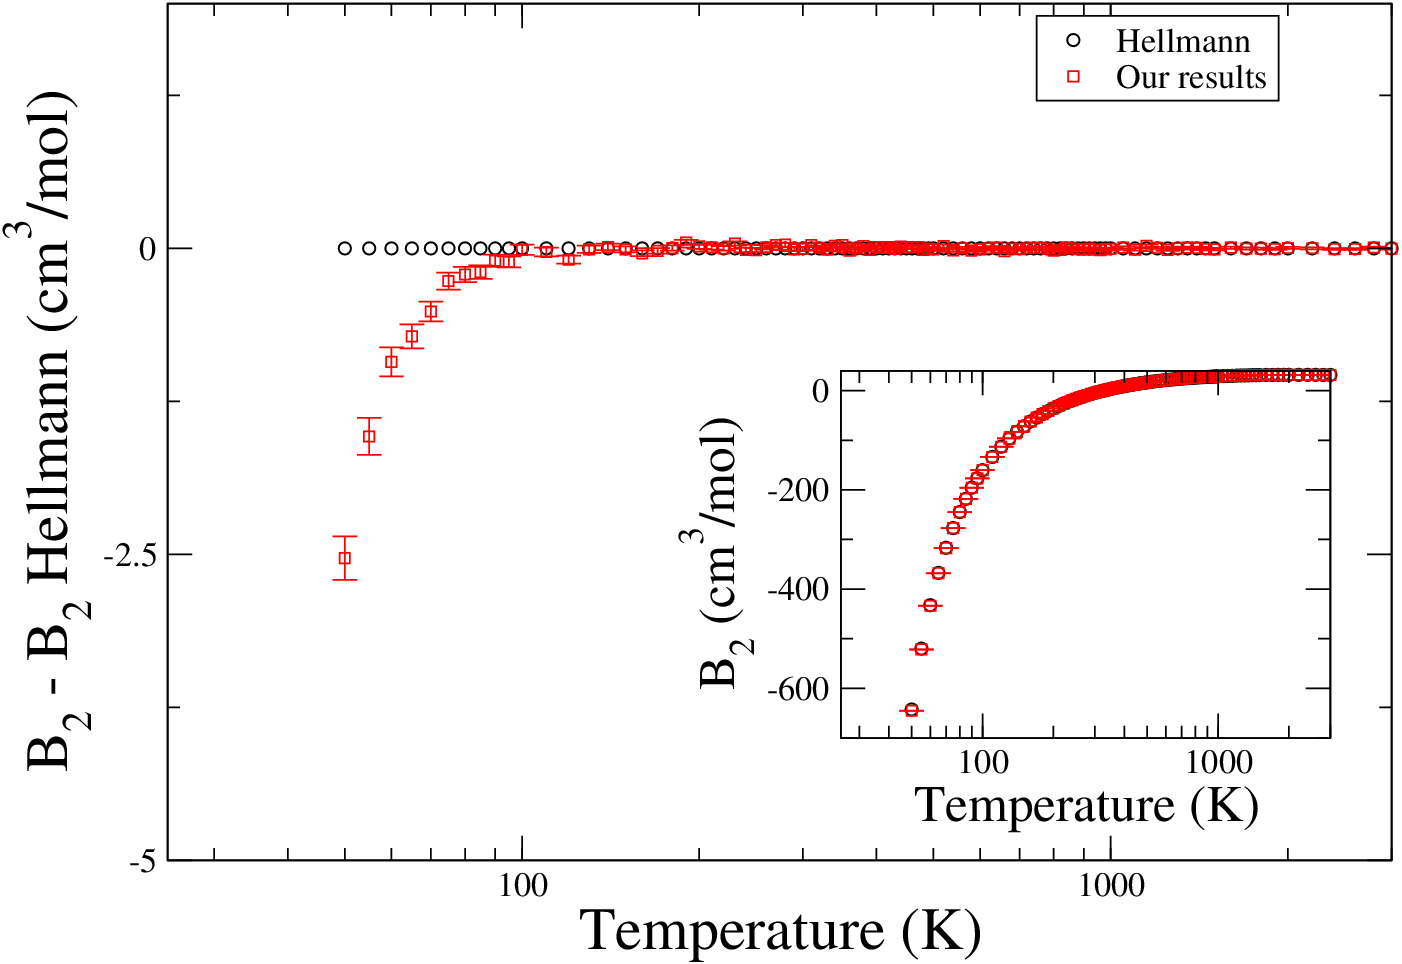
\includegraphics[scale=0.20,keepaspectratio]{Chapter-5/Figures/B2SC9sResultsAll.png}
            \caption{Semi-classical second virial coefficient ($B_2$) values compared against Hellmann's values \cite{Hellmann2013}. Error bars are drawn at $\mu \pm \sigma$ where $\mu$ is the mean value and $\sigma$ is the standard error. It should be noted however, that the 95\% confidence interval is given by $\mu \pm 2\sigma$.}
            \label{fig:B2SCN2}
        \end{figure}
        From Fig. \ref{fig:B2SCN2} and the argument made in Sec. \ref{subsubsec:b2n2}, we can clearly see that our semi-classical results are in excellent agreement with Hellmann's for temperatures $T \ge 100K$. The deviation observed for lower temperatures can be explained by the use of a different semi-classical form of the intermolecular function, i.e., whereas we have used the semi-classical QFH version (Eq. \eqref{eq:QFH}) , Hellmann used the semi-classical TI version (Eq. \eqref{eq:TI}) of the \abinitio{} potential. From Fig. \ref{fig:B2SCN2} one can also make the observation that the semi-classical QFH and the TI versions of the \abinitio{} PES produce similar results until about $T = 100K$ where we start noticing significant deviations.

        In Fig. \ref{fig:B2AllDiffPICB} we plot the differences between the quantum virial coefficient values computed using classical beads and the case of semi-classical beads with $P$ = 64. Under the reasonable assumption that the PI-SCB approach with $P$ = 64 yields the most accurate value, we compare the values computed using PI-CB approaches for different $P$. From Fig. \ref{fig:B2AllDiffPICB}, we can see that there is not much noticeable improvement for the PI-SCB approach over the PI-CB approaches, suggesting that for the purpose quantum virial calculations, we need not resort to PI-SCB approaches.
        \begin{figure}[!htbp]
            \centering
            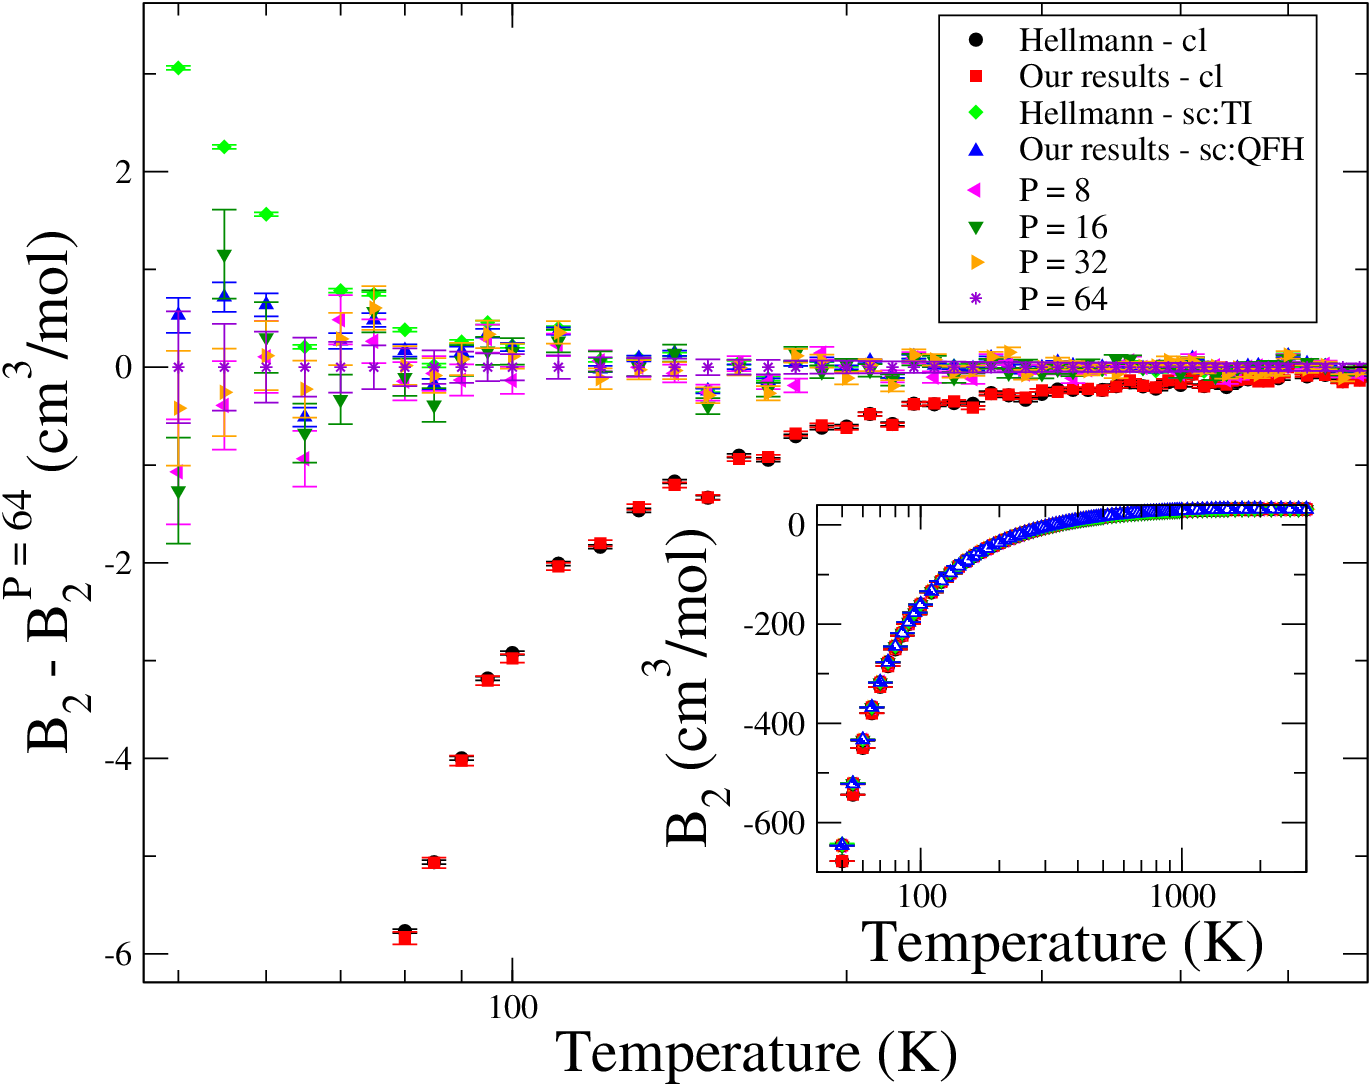
\includegraphics[scale=0.20,keepaspectratio]{Chapter-5/Figures/B2AllDiffPICB.png}
            \caption{Difference between second virial coefficients computed with PI using CB approaches and PI using SCB approach with $P$ = 64 images.}
            \label{fig:B2AllDiffPICB}
        \end{figure}

    \subsection{Third virial coefficients}
        In Figs. \ref{fig:B3CLN2} and \ref{fig:B3SCN2}, we plot the classical and the semi-classical third virial coefficients including additive and non-additive contributions. It should be noted that the range of the $y$-axes were chosen to highlight the differences over the whole range of temperatures considered and as a result we did not include some data points (whose $B_3$ value was lesser than -5 cm$^6$ mol$^{-2}$), especially for low temperatures.
        \begin{figure}[!htbp]
            \centering
            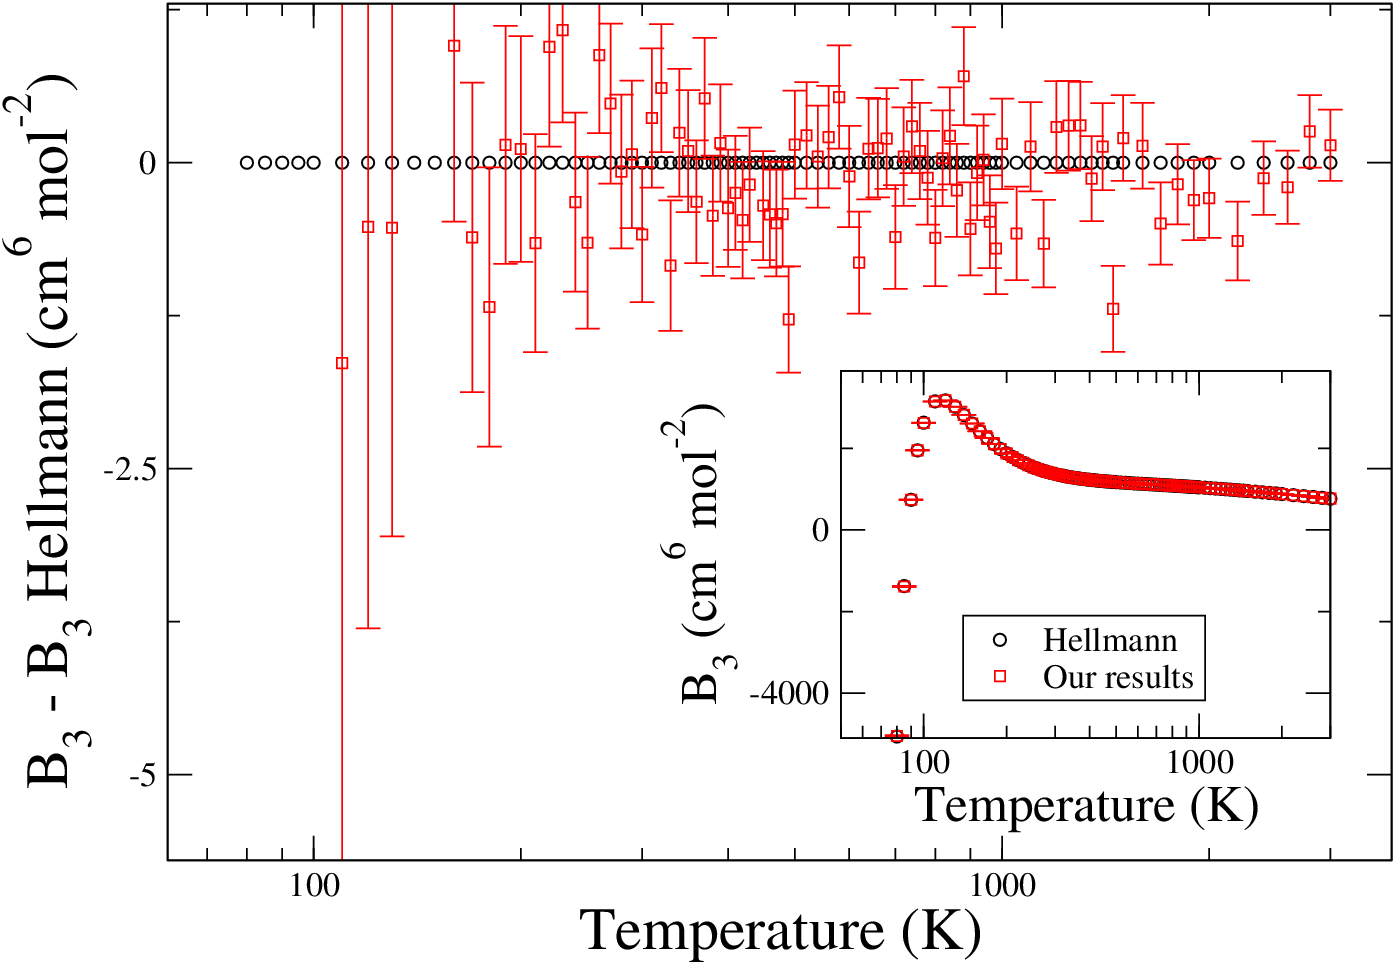
\includegraphics[scale=0.20,keepaspectratio]{Chapter-5/Figures/B3CLFull9sResultsAll.png}
            \caption{Classical second third coefficient ($B_3$) values compared against Hellmann's values \cite{Hellmann2013}. Error bars are drawn at $\mu \pm \sigma$ where $\mu$ is the mean value and $\sigma$ is the standard error. It should be noted however, that the 95\% confidence interval is given by $\mu \pm 2\sigma$.}
            \label{fig:B3CLN2}
        \end{figure}

        \begin{figure}[!htbp]
            \centering
            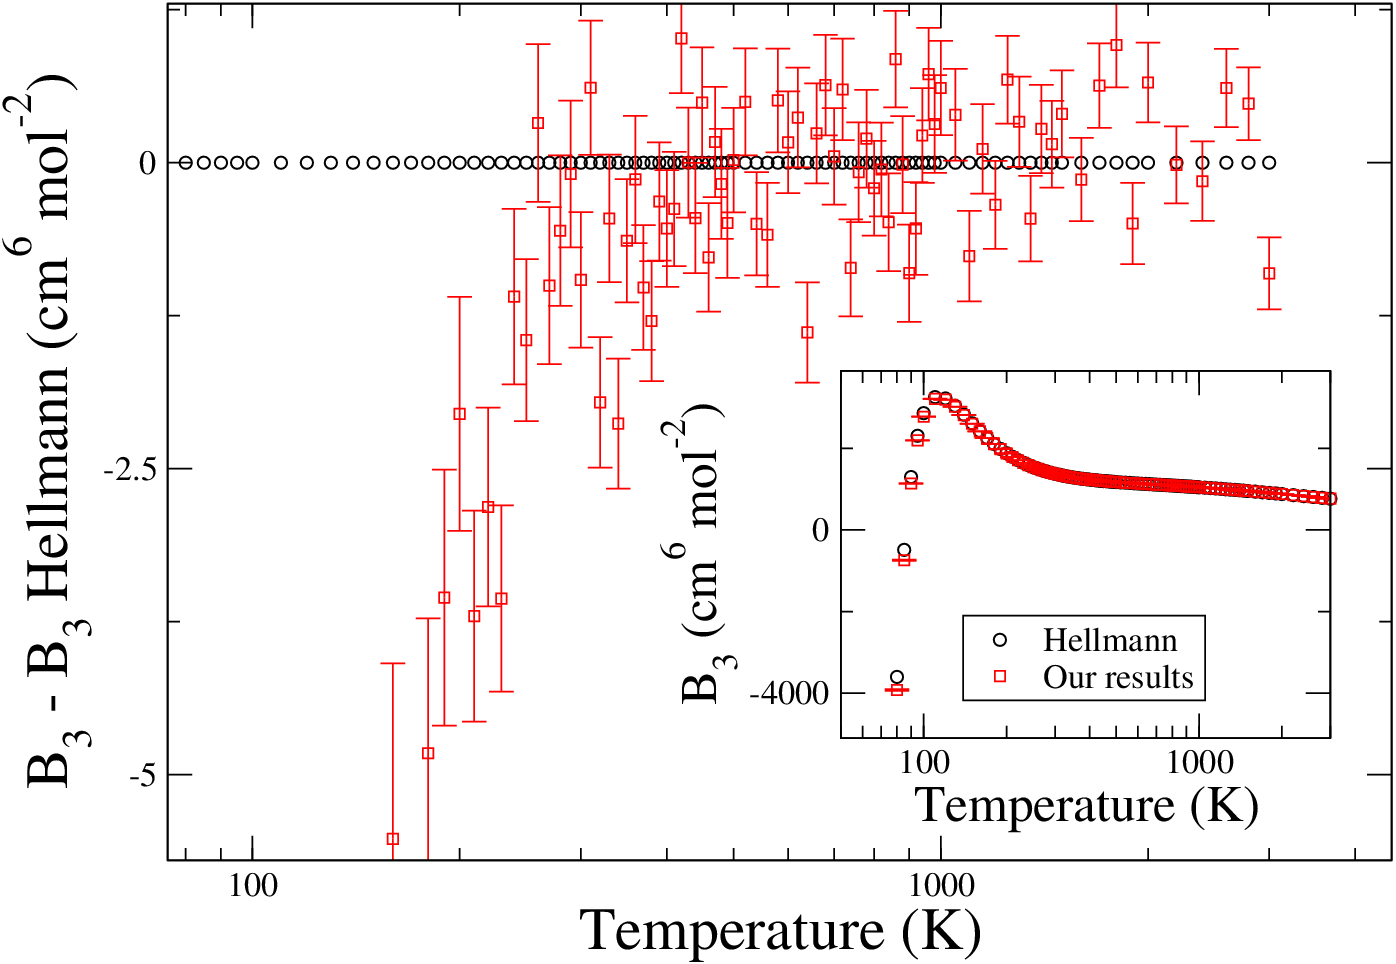
\includegraphics[scale=0.20,keepaspectratio]{Chapter-5/Figures/B3SCFull8sResultsAll.png}
            \caption{Semi-classical third virial coefficient ($B_3$) values compared against Hellmann's values \cite{Hellmann2013}. Error bars are drawn at $\mu \pm \sigma$ where $\mu$ is the mean value and $\sigma$ is the standard error. It should be noted however, that the 95\% confidence interval is given by $\mu \pm 2\sigma$.}
            \label{fig:B3SCN2}
        \end{figure}

        From Fig. \ref{fig:B3CLN2}, we see that our classical $B_3$ results agree quite well with Hellmann's for the entire range of temperatures considered (except a few outliers). The standard error of our results seem to be decreasing with increasing temperature and this is to be expected because any system approaches classical behavior at high enough temperatures. From Fig. \ref{fig:B3SCN2}, we can see that there is quite a bit of deviation of our semi-classical results from Hellmann's corresponding results for $T \le 300K$. As explained earlier, this might be attributed to the use of a different semi-classical form of the \abinitio{} potential. It can also be seen that the deviations become less significant for $T > 300K$. 
        
        In Fig. \ref{fig:B3AllDiffPICB} we plot the differences between the quantum virial coefficient values computed using classical beads and the case of semi-classical beads with $P$ = 64. Under the reasonable assumption that the PI-SCB approach with $P$ = 64 yields the most accurate value, we compare the values computed using PI-CB approaches for different $P$. From Fig. \ref{fig:B3AllDiffPICB}, we can see that there is not much noticeable improvement for the PI-SCB approach over the PI-CB approaches, suggesting that for the purpose quantum virial calculations, we need not resort to PI-SCB approaches.
        \begin{figure}[!htbp]
            \centering
            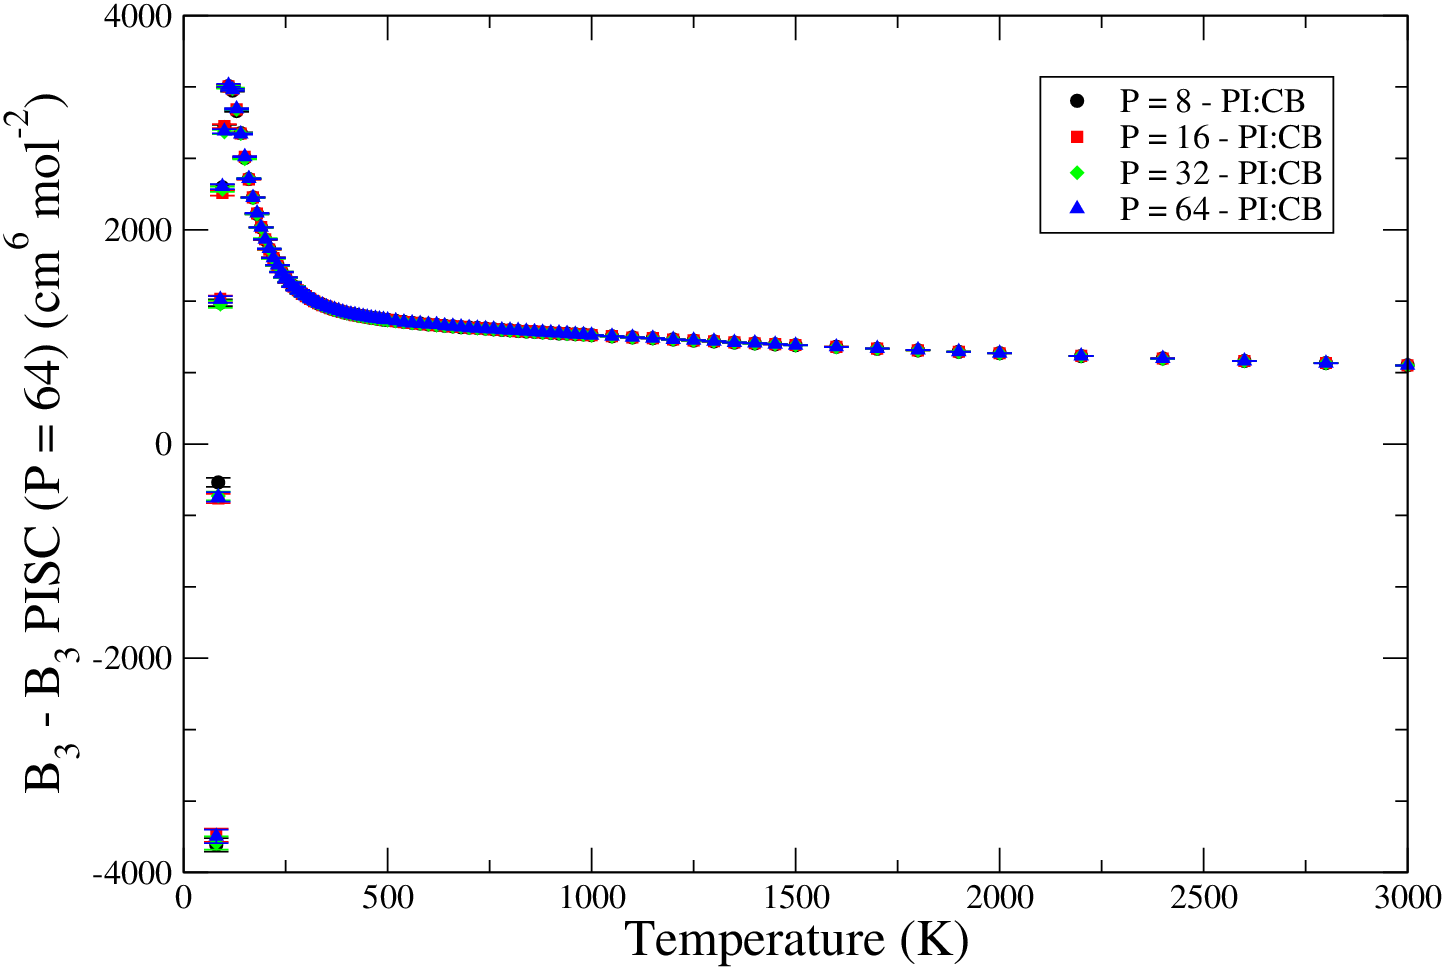
\includegraphics[scale=0.20,keepaspectratio]{Chapter-5/Figures/B3AllDiffPICB.png}
            \caption{Difference between second virial coefficients computed with PI using CB approaches and PI using SCB approach with $P$ = 64 images.}
            \label{fig:B3AllDiffPICB}
        \end{figure}
